\section{eTrice Java Projects}

There are two flavors of \eTrice{} Java projects. The first one uses the Eclipse JDT build and the
second one uses Maven to build and deploy an \eTrice{} application.

The kind of build can be selected in the "Empty eTrice Java project" wizard.

\subsection{Eclipse JDT Build}

If this kind of build is chosen the \eTrice{} new project wizard requires the \texttt{org.eclipse.etrice.runtime.java}
project in the workspace and adds a dependency to it.

If the project uses other \eTrice{} projects (e.g. the \texttt{org.eclipse.etrice.modellib.java})
they have to be added to the Java build path as well.

The \eTrice{} new project wizard creates the following files for the JDT build
\begin{itemize}
\item a ROOM model file with exemplary classes
\item a simple physical model
\item a model mapping the logical entities of the ROOM model to the physical entities
\item a launch configuration that invokes the \eTrice{} Java code generator for the new models
\item a launch configuration that launches the main method of the generated code
\end{itemize}

If "build automatically" is chosen the newly created model can be generated and launched with just two clicks.

\subsection{Maven Build}

The Maven integration of eTrice requires the m2eclipse plug-in installed. The dependencies are then managed
by the Maven pom.xml but the m2e builder maps them as JDT visible dependencies to the project class path.

The \eTrice{} new project wizard creates the following files for the Maven build
\begin{itemize}
\item a ROOM model file with exemplary classes
\item a simple physical model
\item a model mapping the logical entities of the ROOM model to the physical entities
\item a launch configuration that invokes the \eTrice{} Java code generator for the new models
\item a launch configuration that builds and deploys the generated application
\item a launch configuration that launches the deployed jar file
\item a launch configuration that launches the main method of the generated code (for convenience or
if the generated code should be launched in debug mode)
\end{itemize}

After the new project is created the m2e builder creates the dependencies in the project class path.
Therefore also JDT can compile and launch the application.

\subsubsection*{Example}

As an example we want to use the \nameref{sec:ping_pong_tutorial}.

For this example we start with an empty workspace.
We create a new eTrice project using the "Empty eTrice Java Project" wizard which results in a workspace looking
like:

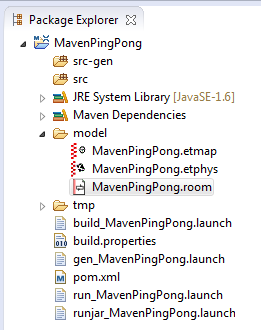
\includegraphics{images/042-after-project-creation.png}

The only difference to the first version of this example is the resolution of the \texttt{TimingService} using
a classpath scheme:

\begin{lstlisting}[language=ROOM]
import room.basic.service.timing.* from "classpath:/TimingService.room"
\end{lstlisting}

It is possible to navigate to the imported model:

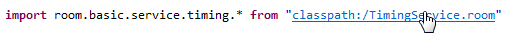
\includegraphics{images/042-navigate-import.png}

but the model is read-only. It is found on the class path of the project which is derived from the project pom's dependencies:

\begin{lstlisting}[language=XML]
<dependency>
	<groupId>org.eclipse.etrice</groupId>
	<artifactId>org.eclipse.etrice.modellib.java</artifactId>
	<version>0.5.0-SNAPSHOT</version>
</dependency>
\end{lstlisting}

Since during the generate-sources life cycle phase the same dependency is needed we have to add it also to
our eTrice generator plug-in:

\begin{lstlisting}[language=XML]
<build>
	<plugins>
		<plugin>
			<groupId>org.eclipse.etrice</groupId>
			<artifactId>org.eclipse.etrice.generator.java.mvn</artifactId>
			<version>0.5.0-SNAPSHOT</version>
			<!-- [...] -->
			<dependencies>
				<!-- put the modellib on the class path to allow resolution of models by the generator -->
				<dependency>
					<groupId>org.eclipse.etrice</groupId>
					<artifactId>org.eclipse.etrice.modellib.java</artifactId>
					<version>0.5.0-SNAPSHOT</version>
				</dependency>
			</dependencies>
		</plugin>
	</plugins>
</build>
\end{lstlisting}

Now we start the build, e.g. by entering \texttt{mvn clean package} on the command line or by launching Maven
using m2e. Maven will download all needed artifacts. The build should succeed and contain somewhere the generator
output:

\begin{lstlisting}[language=PlainText]
[INFO] Info: -- reading models
[INFO] Info: added model model/MavenPingPong.etmap
[INFO] Info: Loading file:/C:/eTrice-mvn-tutorial/MavenPingPong/model/MavenPingPong.etmap
[INFO] Info: added referenced model file:/C:/eTrice-mvn-tutorial/MavenPingPong/model/MavenPingPong.room
[INFO] Info: added referenced model file:/C:/eTrice-mvn-tutorial/MavenPingPong/model/MavenPingPong.etphys
[INFO] Info: Loading file:/C:/eTrice-mvn-tutorial/MavenPingPong/model/MavenPingPong.room
[INFO] Info: added referenced model classpath:/TimingService.room
[INFO] Info: Loading jar:file:/C:/Users/hrentz/.m2/repository/org/eclipse/etrice/org.eclipse.etrice.modellib.java/0.5.0-SNAPSHOT/org.eclipse.etrice.modellib.java-0.5.0-SNAPSHOT.jar!/TimingService.room
[INFO] Info: Loading file:/C:/eTrice-mvn-tutorial/MavenPingPong/model/MavenPingPong.etphys
[INFO] Info: -- validating models
[INFO] Info: validation finished with 0 errors and 0 warnings
[INFO] Info: -- creating generator model
[INFO] Info: GeneratorModelBuilder: creating system class from LogSys1
[INFO] Info: GeneratorModelBuilder: creating subsystem instance from subSysRef1
[INFO] Info: -- starting code generation
[INFO] Info: clearing C:\eTrice-mvn-tutorial\MavenPingPong/src-gen/
[INFO] Info: clearing /src-gen/
[INFO] Info: generating ProtocolClass implementation 'PingPongProtocol.java' in 'C:\eTrice-mvn-tutorial\MavenPingPong/src-gen/MavenPingPong/'
[INFO] Info: generating ActorClass implementation 'PingPongTop.java' in 'C:\eTrice-mvn-tutorial\MavenPingPong/src-gen/MavenPingPong/'
[INFO] Info: generating ActorClass implementation 'Receiver.java' in 'C:\eTrice-mvn-tutorial\MavenPingPong/src-gen/MavenPingPong/'
[INFO] Info: generating ActorClass implementation 'Sender.java' in 'C:\eTrice-mvn-tutorial\MavenPingPong/src-gen/MavenPingPong/'
[INFO] Info: generating Node implementation 'Node_nodeRef1_subSysRef1.java' in 'C:\eTrice-mvn-tutorial\MavenPingPong/src-gen/MavenPingPong/'
[INFO] Info: generating SubSystemRunner implementation 'Node_nodeRef1_subSysRef1Runner.java' in 'C:\eTrice-mvn-tutorial\MavenPingPong/src-gen/MavenPingPong/'
[INFO] Info: -- finished code generation
\end{lstlisting}

When the packaging of the project succeeded two jar files have been created in the \texttt{target} folder.
The larger one with "jar-with-dependencies" in its name also contains the referenced Maven components. It can be
launched using the \texttt{runjar\_*} launch configuration.

Finally we want to mention that the generator switches are passed as arguments to the plug-in.
In the pom you can find the most commonly used ones in xml comments together with a comment:

\begin{lstlisting}[language=XML]
<plugin>
	<groupId>org.eclipse.etrice</groupId>
	<artifactId>org.eclipse.etrice.generator.java.mvn</artifactId>
	<version>0.5.0-SNAPSHOT</version>
	<executions>
		<execution>
			<goals>
				<goal>eTriceJavaGenerator</goal>
			</goals>
			<configuration>
				<arguments>
					<!-- allowed switches for the generator (not complete) -->
					<!-- generate the store/restore interface using POJO data objects
					<param>-storeDataObj</param>
					-->
					<!-- generate MSC instrumentation
					<param>-msc_instr</param>
					-->
					<!-- generate the persistence interface for dynamic actors
					<param>-persistable</param>
					-->
					<!-- generate all ROOM classes as library
					<param>-lib</param>
					-->
					<!-- generate documentation
					<param>-genDocu</param>
					-->
					<!-- generate files incrementally (overwrite only if contents changed)
					<param>-inc</param>
					-->
					<param>model/MavenPingPong.etmap</param>
				</arguments>
			</configuration>
		</execution>
	</executions>
	<dependencies>
		<!-- [...] -->
	</dependencies>
</plugin>
\end{lstlisting}

E.g. for our example you might want to use the \texttt{-msc\_instr} switch to generate MSCs.

Finally for reference we show the complete ROOM model of this example:

\lstinputlisting[language=ROOM, caption={ROOM example code}, label={lst:room_example}]{../model/maven-ping-pong-example.room}
